\documentclass[a4paper]{book}

% Package for setting up A4 size and margins like Word's default
\usepackage[a4paper, margin=2.54cm]{geometry}

% Package for Chinese characters
\usepackage{ctex}

% Package for mathematical formulas
\usepackage{amsmath}
\usepackage{graphicx}
% Package for code highlighting
\usepackage{minted}
\usepackage{listings}
\usepackage{silence}
\WarningFilter{latex}{UTF8}

\usepackage{xcolor}
\usepackage{mdframed}

% \definecolor{green}{RGB}{230, 252, 238}
\definecolor{green}{RGB}{191, 214, 199}

\newmdenv[
backgroundcolor=green,
linecolor=green
]{greenbox}

\begin{document}

\chapter{Processor Scheduling}

\section{Bank's Algorithm}

\begin{greenbox}
There are 5 concurrent processes \(P_1\), \(P_2\), \(P_3\), \(P_4\), \(P_5\).

There are 3 types of resources \(R_1\), \(R_2\), \(R_3\) in the shared system.

The number of resources in \(R_1\), \(R_2\), \(R_3\) is 16, 5, 19 respectively.

Let's use Allocated(\(P_n\), a, b, c) to indicate that the number of resources in \(R_1\), \(R_2\), \(R_3\) allocated to process n is a, b, c respectively.

MaxRequire(\(P_n\), x, y, z) indicates that the maximum resource requirement of process n is (x, y, z).

The system status at time \(T_0\) is as follows:

Allocated(\(P_1\),2,1,2)

Allocated(\(P_2\),4,0,2)

Allocated(\(P_3\),4,0,5)

Allocated(\(P_4\),2,0,4)

Allocated(\(P_5\),3,1,4)

MaxRequire(\(P_1\),5,5,9)

MaxRequire(\(P_2\),5,3,6)

MaxRequire(\(P_3\),4,0,11)

MaxRequire(\(P_4\),4,2,5)

MaxRequire(\(P_5\),3,2,4)

The system adopts the banker's algorithm strategy to avoid deadlock.

Please judge whether the state is safe at time \(T_0\).
\end{greenbox}


有5个并发进程\(P_1\), \(P_2\),\(P_3\), \(P_4\),\(P_5\).

共享系统中有三类资源\(R_1\),\(R_2\),\(R_3\).

\(R_1\),\(R_2\),\(R_3\)的资源数分别是16,5,19.

不妨用Allocated(\(P_n\),a,b,c)表示进程n分配到的\(R_1\),\(R_2\),\(R_3\)的资源数量分别为a,b,c.

MaxRequire(\(P_n\),x,y,z)表示进程n的最大资源需求量为(x,y,z).

在\(T_0\)时刻的系统状态如下所示:

(略)

系统采用的银行家算法的策略避免死锁。请你判断\(T_0\)时刻是否处于安全状态。

The \textbf{Banker's Algorithm} is a method used to determine whether a system is in a \textbf{safe state}, meaning that it can allocate resources to all processes in some order without leading to a deadlock.

To check whether the state at \( T_0 \) is safe, let's proceed step by step:

\hrulefill

\subsubsection{Step 1: Calculate Available Resources}

The total resources in the system are:
\begin{itemize}
\item 
\( R_1 = 16 \)

\item 
\( R_2 = 5 \)

\item 
\( R_3 = 19 \)

\end{itemize}

The total allocated resources (sum of all allocated resources across processes) are:
\begin{itemize}
\item 
\( \text{Allocated} R_1 = 2+4+4+2+3 = 15 \)

\item 
\( \text{Allocated} R_2 = 1+0+0+0+1 = 2 \)

\item 
\( \text{Allocated} R_3 = 2+2+5+4+4 = 17 \)

\end{itemize}

The available resources are:
\begin{itemize}
\item 
\( \text{Available} R_1 = 16 - 15 = 1 \)

\item 
\( \text{Available} R_2 = 5 - 2 = 3 \)

\item 
\( \text{Available} R_3 = 19 - 17 = 2 \)

\end{itemize}

So, \textbf{Available = (1, 3, 2)}.

\hrulefill

\subsubsection{Step 2: Calculate Need Matrix}

The \textbf{Need} for each process is calculated as:
\[
\text{Need}(P_n) = \text{MaxRequire}(P_n) - \text{Allocated}(P_n)
\]

\begin{tabular}{l l}
Process & Need for \( R_1, R_2, R_3 \) \\
\hline
\( P_1 \) & \( (5-2, 5-1, 9-2) = (3, 4, 7) \) \\
\( P_2 \) & \( (5-4, 3-0, 6-2) = (1, 3, 4) \) \\
\( P_3 \) & \( (4-4, 0-0, 11-5) = (0, 0, 6) \) \\
\( P_4 \) & \( (4-2, 2-0, 5-4) = (2, 2, 1) \) \\
\( P_5 \) & \( (3-3, 2-1, 4-4) = (0, 1, 0) \) \\
\end{tabular}

\hrulefill

\subsubsection{Step 3: Check the Safe Sequence}

We now try to find a sequence in which all processes can complete without exceeding the available resources.

\subsubsection{Iteration 1:}
\begin{itemize}
\item 
Available = \( (1, 3, 2) \)

\item 
Check each process:
\begin{itemize}
\item 
\( P_1 \): Needs \( (3, 4, 7) \), cannot be satisfied.

\item 
\( P_2 \): Needs \( (1, 3, 4) \), cannot be satisfied.

\item 
\( P_3 \): Needs \( (0, 0, 6) \), cannot be satisfied.

\item 
\( P_4 \): Needs \( (2, 2, 1) \), cannot be satisfied.

\item 
\( P_5 \): Needs \( (0, 1, 0) \), \textbf{can be satisfied}.

\end{itemize}

\item 
\( P_5 \) completes. After \( P_5 \) releases its allocated resources \( (3, 1, 4) \), the available resources become:
[
(1+3, 3+1, 2+4) = (4, 4, 6)
]

\end{itemize}

\subsubsection{Iteration 2:}
\begin{itemize}
\item 
Available = \( (4, 4, 6) \)

\item 
Check each process:
\begin{itemize}
\item 
\( P_1 \): Needs \( (3, 4, 7) \), cannot be satisfied.

\item 
\( P_2 \): Needs \( (1, 3, 4) \), \textbf{can be satisfied}.

\end{itemize}

\item 
\( P_2 \) completes. After \( P_2 \) releases its allocated resources \( (4, 0, 2) \), the available resources become:
[
(4+4, 4+0, 6+2) = (8, 4, 8)
]

\end{itemize}

\subsubsection{Iteration 3:}
\begin{itemize}
\item 
Available = \( (8, 4, 8) \)

\item 
Check each process:
\begin{itemize}
\item 
\( P_1 \): Needs \( (3, 4, 7) \), \textbf{can be satisfied}.

\end{itemize}

\item 
\( P_1 \) completes. After \( P_1 \) releases its allocated resources \( (2, 1, 2) \), the available resources become:
[
(8+2, 4+1, 8+2) = (10, 5, 10)
]

\end{itemize}

\subsubsection{Iteration 4:}
\begin{itemize}
\item 
Available = \( (10, 5, 10) \)

\item 
Check each process:
\begin{itemize}
\item 
\( P_3 \): Needs \( (0, 0, 6) \), \textbf{can be satisfied}.

\end{itemize}

\item 
\( P_3 \) completes. After \( P_3 \) releases its allocated resources \( (4, 0, 5) \), the available resources become:
[
(10+4, 5+0, 10+5) = (14, 5, 15)
]

\end{itemize}

\subsubsection{Iteration 5:}
\begin{itemize}
\item 
Available = \( (14, 5, 15) \)

\item 
Check each process:
\begin{itemize}
\item 
\( P_4 \): Needs \( (2, 2, 1) \), \textbf{can be satisfied}.

\end{itemize}

\item 
\( P_4 \) completes. After \( P_4 \) releases its allocated resources \( (2, 0, 4) \), the available resources become:
[
(14+2, 5+0, 15+4) = (16, 5, 19)
]

\end{itemize}

\hrulefill

\subsubsection{Step 4: Conclusion}

All processes can finish in the order \( P_5 \rightarrow P_2 \rightarrow P_1 \rightarrow P_3 \rightarrow P_4 \). Since a safe sequence exists, the system is in a \textbf{safe state} at \( T_0 \).

\section{PV Operation - Chicken and Chef}

\begin{greenbox}
There is a cage that can hold up to three chickens. Each time the supplier puts a chicken into the cage, if the cage is full, the supplier must wait. Each time the chef takes a chicken out of the cage, if the cage is empty, he must also wait. Assuming that the cage is empty at the initial moment, define a semaphore and initialize it to use PV operations to achieve synchronization and mutual exclusion between the supplier and the chef.
\end{greenbox}

有一个最多可以装三只鸡的铁笼子。供应商每次向笼子里面放一只鸡,如果笼子是满的,供应商必须等待。 厨师每次从笼子里面取出一只鸡,如果笼子是空的,也必须等待。假设初始时刻笼子是空的,定义信号量并初始化用PV操作实现供应商和厨师之间的同步和互斥.

This scenario is a classic producer-consumer problem where semaphores are used for synchronization and mutual exclusion. Here's how you can define and initialize the semaphores for the given situation:

\subsubsection{Semaphores}
\begin{enumerate}
\item 
\verb|empty|: Tracks the number of empty slots in the cage. Initialize it to 3 (maximum capacity of the cage).

\item 
\verb|full|: Tracks the number of chickens in the cage. Initialize it to 0 (cage is empty initially).

\item 
\verb|mutex|: Ensures mutual exclusion while accessing the cage. Initialize it to 1.

\end{enumerate}

\subsubsection{C Code Using PV Operations}

\begin{minted}[frame=lines, fontsize=\normalsize]{c}
#include <stdio.h>
#include <stdlib.h>
#include <pthread.h>
#include <semaphore.h>
#include <unistd.h>

// Semaphores
sem_t empty;  // Number of empty slots
sem_t full;   // Number of chickens in the cage
sem_t mutex;  // Ensures mutual exclusion

// Supplier function
void *supplier(void *arg) {
    while (1) {
        sem_wait(&empty);      // Wait if there are no empty slots
        sem_wait(&mutex);      // Enter critical section
        printf("Supplier puts a chicken in the cage.\n");
        sem_post(&mutex);      // Exit critical section
        sem_post(&full);       // Increase the count of full slots
        sleep(1);              // Simulate time taken to supply
    }
    return NULL;
}

// Chef function
void *chef(void *arg) {
    while (1) {
        sem_wait(&full);       // Wait if there are no chickens
        sem_wait(&mutex);      // Enter critical section
        printf("Chef takes a chicken from the cage.\n");
        sem_post(&mutex);      // Exit critical section
        sem_post(&empty);      // Increase the count of empty slots
        sleep(1);              // Simulate time taken to cook
    }
    return NULL;
}

int main() {
    // Initialize semaphores
    sem_init(&empty, 0, 3);  // Cage can hold up to 3 chickens
    sem_init(&full, 0, 0);   // Cage is empty initially
    sem_init(&mutex, 0, 1);  // Mutex for critical section

    pthread_t supplier_thread, chef_thread;

    // Create threads for supplier and chef
    pthread_create(&supplier_thread, NULL, supplier, NULL);
    pthread_create(&chef_thread, NULL, chef, NULL);

    // Wait for threads to finish (they won't, as this runs indefinitely)
    pthread_join(supplier_thread, NULL);
    pthread_join(chef_thread, NULL);

    // Destroy semaphores
    sem_destroy(&empty);
    sem_destroy(&full);
    sem_destroy(&mutex);

    return 0;
}
\end{minted}

\subsubsection{Explanation}
\begin{enumerate}
\item 
\verb|sem_wait()| (P operation): Decrements the semaphore. If the semaphore's value is zero, the calling thread blocks until it becomes positive.

\item 
\verb|sem_post()| (V operation): Increments the semaphore and wakes up one of the waiting threads, if any.

\end{enumerate}

\subsubsection{Synchronization Steps}
\begin{itemize}
\item 
The \textbf{supplier}:
\begin{itemize}
\item 
Waits (\verb|sem_wait(&empty)|) until there is at least one empty slot in the cage.

\item 
Enters the critical section using \verb|mutex| to safely add a chicken to the cage.

\item 
Signals (\verb|sem_post(&full)|) that a chicken is now available.

\end{itemize}

\item 
The \textbf{chef}:
\begin{itemize}
\item 
Waits (\verb|sem_wait(&full)|) until there is at least one chicken in the cage.

\item 
Enters the critical section using \verb|mutex| to safely take a chicken from the cage.

\item 
Signals (\verb|sem_post(&empty)|) that a slot in the cage is now empty.

\end{itemize}

\end{itemize}

Here is a concise pseudocode for the core part:

\begin{minted}[frame=lines, fontsize=\normalsize]{c}
// Supplier
supplier() {
    while (true) {
        P(empty);          // Wait for an empty slot
        P(mutex);          // Enter critical section
        // Add a chicken to the cage
        V(mutex);          // Exit critical section
        V(full);           // Signal a full slot
    }
}

// Chef
chef() {
    while (true) {
        P(full);           // Wait for a full slot
        P(mutex);          // Enter critical section
        // Take a chicken from the cage
        V(mutex);          // Exit critical section
        V(empty);          // Signal an empty slot
    }
}
\end{minted}

\subsubsection{Explanation of Operations}
\begin{itemize}
\item 
\verb|P(semaphore)|: Wait (decrement semaphore).

\item 
\verb|V(semaphore)|: Signal (increment semaphore).

\end{itemize}

\subsubsection{Semaphores Initialization}

\begin{lstlisting}[language=c]
// Initialization:
sem_init(&empty, 0, 3);  // Cage capacity
sem_init(&full, 0, 0);   // Initially empty
sem_init(&mutex, 0, 1);  // For mutual exclusion
\end{lstlisting}

This pseudocode simplifies the logic for synchronization and mutual exclusion.

This approach ensures both synchronization (supplier and chef waiting for their turn) and mutual exclusion (only one thread accessing the cage at a time).

\chapter{Memory Management}

\section{Memory Allocation}

\subsection{Virtual Memory}

\begin{greenbox}
The virtual address of a job is 24 bits. The upper 8 bits are the segment number, and the lower 16 bits are the relative address within the segment.
Please give the calculation process in detail for the following 3 calculation questions:

1. How many segments can a job have at most?

2. What is the maximum length of each segment?

3. The following table is a segment table used by a segment storage management

\vspace{0.5cm}
\begin{tabular}{|c|c|p{3cm}|p{3cm}|}
    \hline
    Segment number & segment length & main memory\newline start address & whether in\newline main memory \\ \hline
    0   & 600   & 2100  & Yes \\ \hline
    1   & 40    & 2800  & Yes \\ \hline
	2   & 100   & N/A   & No  \\ \hline
	3   & 80    & 4000  & Yes \\ \hline
\end{tabular}
\vspace{0.5cm}

Please calculate the main memory addresses of [0, 430], [1, 50], [2, 30], [3, 70]. The first value in the square brackets is the segment number, and the second value is the address within the segment. When address conversion is not possible, please explain what kind of interrupt is generated.
\end{greenbox}

Let's go through the three questions step by step with detailed explanations.

\textbf{How many segments can a job have at most?}

The virtual address of the job is 24 bits. The upper 8 bits represent the \textbf{segment number}, and the lower 16 bits represent the \textbf{relative address within the segment}. This means:

- The \textbf{segment number} is represented by 8 bits.

- The \textbf{relative address} within the segment is represented by 16 bits.

Now, the question asks how many segments a job can have at most. Since the \textbf{segment number} is represented by 8 bits, the number of distinct values the segment number can take is:

\[
2^8 = 256
\]

Thus, the job can have at most \textbf{256 segments}.

\textbf{What is the maximum length of each segment?}

The maximum length of a segment corresponds to the maximum value of the \textbf{relative address} within the segment, which is represented by the \textbf{lower 16 bits}. The maximum value that can be represented by 16 bits is:

\[
2^{16} - 1 = 65535
\]

So, the maximum length of each segment is \textbf{65535} units (e.g., bytes, words, etc.), which is the highest relative address that can be represented with 16 bits.

\textbf{Memory address calculations from the segment table}

Given the segment table:

\vspace{0.5cm}
\begin{tabular}{|c|c|p{3cm}|p{3cm}|}
    \hline
    Segment number & segment length & main memory start address & whether in main memory \\ \hline
    0   & 600   & 2100 & Yes  \\  \hline
    1   & 40    & 2800 & Yes  \\  \hline
	2   & 100   & N/A  & No   \\  \hline
	3   & 80    & 4000 & Yes  \\  \hline
\end{tabular}

We need to calculate the main memory address for each of the following cases:

- \textbf{[0, 430]}: Segment 0, relative address 430

- \textbf{[1, 50]}: Segment 1, relative address 50

- \textbf{[2, 30]}: Segment 2, relative address 30

- \textbf{[3, 70]}: Segment 3, relative address 70

\textbf{Calculations:}

\textit{\textbf{1. \textbf{[0, 430]}: Segment 0, relative address 430}}

- Segment 0 starts at main memory address 2100 and has a length of 600.

- The main memory address is calculated by adding the relative address (430) to the start address of the segment (2100):
  
\[
\text{Main Memory Address} = 2100 + 430 = 2530
\]

So, the main memory address for \textbf{[0, 430]} is \textbf{2530}.

\textit{\textbf{2. \textbf{[1, 50]}: Segment 1, relative address 50}}

- Segment 1 starts at main memory address 2800 and has a length of 40.

- The main memory address is calculated by adding the relative address (50) to the start address of the segment (2800):
  
\[
\text{Main Memory Address} = 2800 + 50 = 2850
\]

However, the segment length of Segment 1 is only 40, so the relative address 50 exceeds the segment’s size. This will cause an \textbf{interrupt} due to a \textbf{segmentation fault}, as the address is outside the bounds of the segment.

\textit{\textbf{3. \textbf{[2, 30]}: Segment 2, relative address 30}}

- Segment 2 is \textbf{not in main memory} (its main memory start address is N/A), which means it is \textbf{not accessible} right now.

- An \textbf{interrupt} will be generated for this address request because the segment is not in memory, likely triggering a \textbf{page fault} or a \textbf{segmentation fault}, depending on the system's memory management.

\textit{\textbf{4. \textbf{[3, 70]}: Segment 3, relative address 70}}

- Segment 3 starts at main memory address 4000 and has a length of 80.

- The main memory address is calculated by adding the relative address (70) to the start address of the segment (4000):
  
\[
\text{Main Memory Address} = 4000 + 70 = 4070
\]

So, the main memory address for \textbf{[3, 70]} is \textbf{4070}.

\textbf{Summary of Results}

\vspace{0.5cm}
\begin{tabular}{|c|c|p{4cm}|c|}
    \hline
    Segment Number & Relative Address & Resulting\newline Main Memory Address & Explanation \\ \hline
    0   & 430   & 2530  & Valid address \\ \hline
    1   & 50    & Error\newline(segmentation fault)  & Address exceeds \\ \hline
	2   & 30   & Error\newline(not in memory) & Segment not in memory  \\ \hline
	3   & 70    & 4070  & Valid address \\ \hline
\end{tabular}

\textbf{Interrupts:}

- For \textbf{[1, 50]}, a segmentation fault occurs because the relative address exceeds the segment's length.

- For \textbf{[2, 30]}, an interrupt occurs because the segment is not in memory.

\newpage

\subsection{Allocation Algorithm}

\begin{greenbox}
There are three jobs, A (30K), B (70K) and C (50K), which request memory allocation in sequence. There are two non-contiguous free areas in the memory, F1 (100K) and F2 (50K). Please use the best fit algorithm and the worst fit algorithm to explain the memory allocation process.

In memory management, \textbf{Best Fit} and \textbf{Worst Fit} are two allocation strategies used to assign free memory areas to processes. Let's walk through the allocation process for both algorithms based on the given scenario:
\end{greenbox}

\begin{figure}[h]
    \centering
    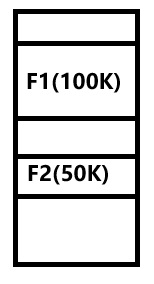
\includegraphics[height=5cm]{img/memory-virtual_memory.jpg}  % Adjust width as needed
    \caption{Your Image Caption}
    \label{fig:your_label}
\end{figure}

\textbf{Given:}

- \textbf{Jobs}:

  - A (30K)
  
  - B (70K)
  
  - C (50K)
  
- \textbf{Free Memory Areas}:

  - F1 (100K)
  
  - F2 (50K)

\subsubsection{Best Fit Algorithm}

In the \textbf{Best Fit} algorithm, we allocate the memory from the smallest free block that is large enough to satisfy the request. The goal is to leave the smallest leftover space after allocation.

\textit{\textbf{Steps:}}

1. \textbf{Allocate Job A (30K)}:

   - Available memory: F1 (100K), F2 (50K).
   
   - Best Fit chooses the smallest free area that can accommodate the job, which is \textbf{F2 (50K)}.
   
   - \textbf{F2} is reduced to 20K after allocating 30K for Job A.

   New memory areas:
   
   - F1 (100K)
   
   - F2 (20K)

2. \textbf{Allocate Job B (70K)}:

   - Available memory: F1 (100K), F2 (20K).
   
   - Best Fit chooses \textbf{F1 (100K)}, because it is the smallest block that fits Job B.
   
   - \textbf{F1} is reduced to 30K after allocating 70K for Job B.

   New memory areas:
   
   - F1 (30K)
   
   - F2 (20K)

3. \textbf{Allocate Job C (50K)}:

   - Available memory: F1 (30K), F2 (20K).
   
   - There is \textbf{no sufficient memory} left to allocate Job C because neither F1 nor F2 can fit 50K.
   
   - Allocation for Job C fails.

   Final memory allocation:
   
   - Job A allocated to F2 (30K used).
   
   - Job B allocated to F1 (70K used).
   
   - Job C \textbf{cannot be allocated} due to insufficient space.

\subsubsection{Worst Fit Algorithm}

In the \textbf{Worst Fit} algorithm, we allocate the memory from the largest free block, hoping to leave the largest possible remaining space after allocation.

\textit{\textbf{Steps:}}

1. \textbf{Allocate Job A (30K)}:

   - Available memory: F1 (100K), F2 (50K).
   
   - Worst Fit chooses \textbf{F1 (100K)}, because it is the largest free block.
   
   - \textbf{F1} is reduced to 70K after allocating 30K for Job A.

   New memory areas:
   
   - F1 (70K)
   
   - F2 (50K)

2. \textbf{Allocate Job B (70K)}:

   - Available memory: F1 (70K), F2 (50K).
   
   - Worst Fit chooses \textbf{F1 (70K)}, because it is the largest free block.
   
   - \textbf{F1} is reduced to 0K after allocating 70K for Job B.

   New memory areas:
   
   - F1 (0K)
   
   - F2 (50K)

3. \textbf{Allocate Job C (50K)}:

   - Available memory: F2 (50K).
   
   - Worst Fit chooses \textbf{F2 (50K)}, which exactly fits Job C.
   
   - \textbf{F2} is reduced to 0K after allocating 50K for Job C.

   Final memory allocation:
   
   - Job A allocated to F1 (30K used).
   
   - Job B allocated to F1 (70K used).
   
   - Job C allocated to F2 (50K used).

\subsubsection{Summary of Results}

- \textbf{Best Fit}:

  - Job A allocated to F2.
  
  - Job B allocated to F1.
  
  - Job C cannot be allocated.

- \textbf{Worst Fit}:

  - Job A allocated to F1.
  
  - Job B allocated to F1.
  
  - Job C allocated to F2.

In this case, the \textbf{Worst Fit} algorithm results in better memory utilization because all jobs are allocated successfully, whereas \textbf{Best Fit} fails to allocate the third job (C).

\chapter{I/O Management}

\section{Disk}

\subsection{Allocation Algorithm}

\begin{greenbox}
Assume that a hard disk has 200 tracks. The tracks are numbered 0-199. After the head has completed service on track 140, it is now performing read/write operations on track 143. There is the following request sequence in chronological order:
88, 147, 91, 177, 94, 150, 102, 175, 130.

Give the disk request service order, the number of tracks moved, and the average number of tracks moved when using SSTF and SCAN strategies.
\end{greenbox}

假设某硬盘共有200个磁道。磁道编号是0-199. 磁头在140道完成服务后,现在正在143道上进行读/写操作。有如下按时间先后顺序排列的请求序列:
88, 147, 91, 177, 94, 150, 102, 175, 130.

给出用SSTF和SCAN策略时的磁盘请求服务次序、移动磁道数以及平均移动磁道数。

To solve this, we need to determine the order of service for the disk requests using both the SSTF (Shortest Seek Time First) and SCAN (elevator) disk scheduling algorithms, and calculate the total and average number of tracks moved.

\subsubsection{1. \textbf{Shortest Seek Time First (SSTF)}}

- \textbf{Initial position of the head}: Track 143

- \textbf{Request queue}: 88, 147, 91, 177, 94, 150, 102, 175, 130


\textbf{SSTF Strategy}:
This strategy services the request that is closest to the current head position.

\textbf{Execution}:

1. Starting at track 143, the closest request is 147 (distance = 4).
2. Next, from 147, the closest request is 150 (distance = 3).
3. From 150, the closest request is 130 (distance = 20).
4. From 130, the closest request is 102 (distance = 28).
5. From 102, the closest request is 94 (distance = 8).
6. From 94, the closest request is 91 (distance = 3).
7. From 91, the closest request is 88 (distance = 3).
8. From 88, the closest request is 175 (distance = 87).
9. From 175, the closest request is 177 (distance = 2).

\textbf{Service Order}: 143 → 147 → 150 → 130 → 102 → 94 → 91 → 88 → 175 → 177

\textbf{Tracks moved}:

- Total tracks moved: \(4 + 3 + 20 + 28 + 8 + 3 + 3 + 87 + 2 = 158\)

- Average number of tracks moved: \(\frac{158}{9} \approx 17.56\)


\subsubsection{2. \textbf{SCAN (Elevator)}}

- \textbf{Initial position of the head}: Track 143

- \textbf{Request queue}: 88, 147, 91, 177, 94, 150, 102, 175, 130

- \textbf{Direction}: Assume the head moves in the increasing track direction first.


\textbf{SCAN Strategy}:
This strategy moves the head in one direction, servicing all requests until it reaches the end or the last request in that direction, then reverses and services requests in the opposite direction.

\textbf{Execution}:

1. From 143, the head moves right to 147.
2. Then, it continues to 150.
3. Next, it moves to 175 and then to 177 (the end of the right side).
4. The head reverses direction and services requests in decreasing order: 130, 102, 94, 91, and finally 88.

\textbf{Service Order}: 143 → 147 → 150 → 175 → 177 → 130 → 102 → 94 → 91 → 88

\textbf{Tracks moved}:

- Tracks moved in the increasing direction: \(4 + 3 + 25 + 2 = 34\)

- Tracks moved in the decreasing direction: \(47 + 28 + 8 + 3 + 3 = 89\)

- Total tracks moved: \(34 + 89 = 123\)

- Average number of tracks moved: \(\frac{123}{9} \approx 13.67\)


\subsubsection{\textbf{Summary}:}

- \textbf{SSTF}:

  
  - \textbf{Order}: 143 → 147 → 150 → 130 → 102 → 94 → 91 → 88 → 175 → 177

  - \textbf{Total tracks moved}: 158

  - \textbf{Average}: ~17.56 tracks


- \textbf{SCAN}:

  
  - \textbf{Order}: 143 → 147 → 150 → 175 → 177 → 130 → 102 → 94 → 91 → 88

  - \textbf{Total tracks moved}: 123

  - \textbf{Average}: ~13.67 tracks


Certainly! Let's illustrate how the \textbf{FCFS (First-Come, First-Served)} and \textbf{CSCAN (Circular SCAN)} disk scheduling algorithms would process this example.

\begin{greenbox}
Furthermore, illustrating FCFS and CSCAN
\end{greenbox}

\subsubsection{Initial Data:}

- \textbf{Initial position of the head}: Track 143

- \textbf{Request sequence}: 88, 147, 91, 177, 94, 150, 102, 175, 130


\subsubsection{1. \textbf{First-Come, First-Served (FCFS)}}

\textbf{Strategy}:
This algorithm services the requests in the exact order they arrive, without any reordering.

\textbf{Execution}:

- The service order will be: 143 → 88 → 147 → 91 → 177 → 94 → 150 → 102 → 175 → 130.


\textbf{Tracks moved}:

- Total tracks moved:

  
  - From 143 to 88: \(143 - 88 = 55\)

  - From 88 to 147: \(147 - 88 = 59\)

  - From 147 to 91: \(147 - 91 = 56\)

  - From 91 to 177: \(177 - 91 = 86\)

  - From 177 to 94: \(177 - 94 = 83\)

  - From 94 to 150: \(150 - 94 = 56\)

  - From 150 to 102: \(150 - 102 = 48\)

  - From 102 to 175: \(175 - 102 = 73\)

  - From 175 to 130: \(175 - 130 = 45\)


- \textbf{Total tracks moved}: \(55 + 59 + 56 + 86 + 83 + 56 + 48 + 73 + 45 = 561\)


- \textbf{Average number of tracks moved}: \(\frac{561}{9} \approx 62.33\)


\subsubsection{2. \textbf{Circular SCAN (CSCAN)}}

\textbf{Strategy}:
CSCAN works like SCAN but, when the head reaches the end of the disk, it jumps directly to the other end and continues servicing requests in the same direction.

\textbf{Assumption}:

- The head moves in the increasing track direction first (rightwards).


\textbf{Execution}:

1. From track 143, the head moves right to service 147.
2. Then it continues to 150, 175, and 177 (the end of the increasing side).
3. After reaching the highest track (or the last request in that direction), it jumps to track 0 and continues servicing requests from there in the same direction.
4. Services 88, 91, 94, 102, and 130 as it moves up.

\textbf{Service Order}: 143 → 147 → 150 → 175 → 177 → (jump to 0) → 88 → 91 → 94 → 102 → 130

\textbf{Tracks moved}:

- Tracks moved in the increasing direction: \(4 + 3 + 25 + 2 = 34\)

- Jump from 177 to 0: \(177\) (full disk jump)

- Tracks moved from 0 to 88: \(88\)

- Tracks moved to service 91, 94, 102, and 130 sequentially:

  - \(91 - 88 = 3\)

  - \(94 - 91 = 3\)

  - \(102 - 94 = 8\)

  - \(130 - 102 = 28\)


\textbf{Total tracks moved}:

- \(34 + 177 + 88 + 3 + 3 + 8 + 28 = 341\)


\textbf{Average number of tracks moved}:

- \(\frac{341}{9} \approx 37.89\)


\subsubsection{\textbf{Summary}:}

- \textbf{FCFS}:

  
  - \textbf{Order}: 143 → 88 → 147 → 91 → 177 → 94 → 150 → 102 → 175 → 130

  - \textbf{Total tracks moved}: 561

  - \textbf{Average}: ~62.33 tracks


- \textbf{CSCAN}:

  
  - \textbf{Order}: 143 → 147 → 150 → 175 → 177 → (jump to 0) → 88 → 91 → 94 → 102 → 130

  - \textbf{Total tracks moved}: 341

  - \textbf{Average}: ~37.89 tracks


These results illustrate how FCFS tends to result in larger overall movement, while CSCAN, with its uniform sweeping motion and jump, offers more consistent service with fewer tracks moved on average.


\end{document}